\documentclass{article}
\usepackage{fullpage,amsmath,amsthm,graphicx,enumitem,amsfonts}
\usepackage{multicol}
\usepackage{booktabs}
\usepackage{algorithm}
\usepackage{algpseudocode}

\usepackage{tikz}
\usetikzlibrary{positioning, shapes, arrows, fit}

\theoremstyle{definition}
\newtheorem{thm}{Theorem}
\newtheorem{question}[thm]{Question}
\newenvironment{solution}{\noindent\textit{Solution:}}{}

\title{ASEN 5264 Decision Making under Uncertainty\\
       Exam 2: Online Methods and Reinforcement Learning}

\date{\small 
    \textbf{Instructions:} Clearly indicate your final answers and briefly justify numerical answers with text or mathematical expressions. If you do not understand how to do a problem, skip it and move on so that you have time to attempt all problems. You may consult any static source, but you may NOT communicate with any person except the instructor or TA, and you may not use LLMs such as ChatGPT.
}

\begin{document}
\maketitle

% \noindent\textbf{Important:} Please include the following statement along with your signature (typed or handwritten) on the exam: \textbf{``I affirm that I completed this exam without the use of any artificial intelligence tool such as ChatGPT or Github Copilot.''}

\begin{question} (10 pts)
    Suppose that we are using Q-learning to solve an MDP with $S = \{1, 2\}$ and $A = \{\text{a}, \text{b}\}$. The current Q values are given in the table below:
    \begin{center}
        \begin{tabular}{cc|cc}
            \toprule
            $s$ & $a$ & $Q(s, a)$ \\
            \midrule
            1 & a & 5 \\
            1 & b & 3 \\
            2 & a & 4 \\
            2 & b & 2 \\
            \bottomrule
        \end{tabular}
    \end{center}
    If we take step $(s=1, a=\text{a}, s'=2, r=6)$ and use the Q-learning update rule with $\alpha = 0.1$ and $\gamma = 0.9$, which Q values are changed and what are their new values?
\end{question}
\noindent \textbf{Solution: }
Because we gained experience for s = 1 and $a$ = a, the value for Q(s = 1, $a$ = a) will be updated. Following the Q-learning algorithm,
\begin{align*}
    Q(s,a) &\leftarrow Q(s,a) + \alpha\left(r + \gamma \cdot\max_{a'}Q(s',a') - Q(s,a)\right)\\
    Q(s=1,a=\text{a}) &\leftarrow 5 + 0.1\left(6 + 0.9\cdot \max_{a'}Q(s=2,a') - Q(s=1,a=\text{a})\right)\\
    Q(s=1,a=\text{a}) &\leftarrow 5 + 0.1\left(6 + 0.9\cdot Q(s=2,a = \text{a}) - Q(s=1,a=\text{a})\right)\\
    Q(s=1,a=\text{a}) &\leftarrow 5 + 0.1\left(6 + 0.9\cdot4 - 5\right)\\
    Q(s=1,a=\text{a}) &\leftarrow \boxed{5.46}\\
\end{align*}
% \begin{question}
% \end{question}

\clearpage

\begin{question} (20 pts)
    Consider a three-armed Bernoulli bandit with win probabilities $\theta = [0.3, 0.7, 0.4]$. After 10 pulls of each arm, the number of wins for each arm is $w = [2, 5, 6]$.
    \begin{enumerate}[label=(\alph*)]
        \item What is the probability that the next pull will result in a win (+1 reward) if an epsilon greedy policy is used with $\epsilon = 0.1$? Briefly justify your answer.
        \\ \\ \noindent \textbf{Solution: }\\
        The greedy approximation of the success probability $\rho_a = \frac{\text{number of wins } + 1}{\text{number of pulls } + 1}$ are calculated for each arm.
        \begin{align*}
            \rho_1 &= \frac{2 + 1}{10 + 1} = \frac{3}{11}\\
            \rho_2 &= \frac{5 + 1}{10 + 1} = \frac{6}{11}\\
            \rho_3 &= \frac{6 + 1}{10 + 1} = \frac{7}{11}\\
        \end{align*}
        The $\epsilon$-greedy policy will choose the arm with the highest $\rho$ with a probability $1 -\epsilon$, and randomly otherwise. Thus, the probability of winning on the next pull is equal to the following.
        \begin{align*}
            P_{win} &= (1 - \epsilon)\theta_3 + \epsilon\bar{\theta}\\
            &= (1 - 0.1)0.4 + 0.1\frac{0.3 + 0.7 + 0.4}{3}\\
            &= 0.40\bar{6}
        \end{align*}
        \item What is the probability that the next pull will result in a win (+1 reward) if a UCB policy is used with $c = 1$? Briefly justify your answer.
        \\ \\ \noindent \textbf{Solution: }\\
        The Upper Confidence Bound (UCB) equation is given below.
        \begin{equation*}
            \text{UCB}(a) = \rho_a + c\sqrt{\frac{\log{N}}{N(a)}}
        \end{equation*}
        Because all arms have been pulled 10 times, the exploration term $c\sqrt{\frac{\log{N}}{N(a)}}$ is the same for all arms, reducing the policy to the argmax of $\rho_a$. Thus, the policy will result in pulling arm 3, which has a probability of $0.4$ to win. 
        \item After a very large number of pulls, which policy will have the highest average payoff? epsilon-greedy or UCB? Briefly justify your answer.
        \\ \\ \noindent \textbf{Solution: }\\
        In the limit as the number of pulls goes to infinity, the UCB policy converges to the optimal $\theta^*$ value, since the exploration term will converge to zero. However, if $\epsilon$ remains fixed, the $\epsilon$-greedy policy will not converge to the optimal $\theta^*$ value because there will always be an $\epsilon$ chance of choosing a suboptimal arm. Thus, the UCB policy will have the highest average payoff.
    \end{enumerate}
\end{question}

\clearpage

\begin{question} (20 pts)
    Consider a candidate reinforcement learning algorithm for MDPs with integer states and actions that keeps track of a large table, $Q$, where each row corresponds to a state and each column to an action. Let $Q[s, a]$ be the entry in row $s$ and column $a$.
    The algorithm works as follows: 
    \\
    \begin{algorithmic}[1]
        \State Initialize $Q$ to be a matrix of zeros.
        \State Initialize $s$ to be the initial state.
        % \State Initialize $R$ to 0.
        \Loop
            \State $a \gets \text{argmax}\, Q[s, a]$ (Break ties randomly).
            \State Take action $a$, receive reward $r$, and observe the next state $s'$.
            \State $Q[s, a] \gets Q[s, a] + 0.1 (r - Q[s, a])$
            \State $s \gets s'$
            \If{$s$ is a terminal state}
                \State Reset $s$ to the initial state.
            \EndIf
        \EndLoop
    \end{algorithmic}

    \begin{enumerate}[label=(\alph*)]
        \item Should this algorithm be considered model-based or model-free? Why?
        \\ \\ \noindent \textbf{Solution: } This algorithm is ``model free'' because it does not learn an MDP model (the reward and transition distributions) to solve, but instead directly estimates a function $Q$ that the policy is based on. \\
        \item Should this algorithm be considered on-policy or off-policy? Why?
        \\ \\ \noindent \textbf{Solution:} This is an ``on-policy'' algorithm because updates to the learned model, $Q$, use only data from the current policy.\\
        \item What is a major limitation of this algorithm related to exploration? Briefly justify your answer.
        \\ \\ \noindent \textbf{Solution: } the policy always takes the action that maximizes $Q$ and only explores randomly if there is a tie. This would make the algorithm susceptible to reaching a local optimum and never exploring other policies. \\
        \item What is a major limitation of this algorithm related to credit assignment? Briefly justify your answer.
        \\ \\ \noindent \textbf{Solution: } This algorithm learns a $Q$ function that only takes the immediate reward for a state and action into account - it cannot learn a value function that includes the long-term consequences of an action. \\
    \end{enumerate}
\end{question}

\clearpage
\begin{question} (20 pts)
    Consider the following MCTS tree where state nodes are represented with circles and action nodes with squares. States are represented with integers and there are two actions, a and b. If the generative function is called at any point, use the values in the table to the right and use a discount of $\gamma=0.9$ if needed.\\
    \\
    \begin{minipage}{0.5\textwidth}
    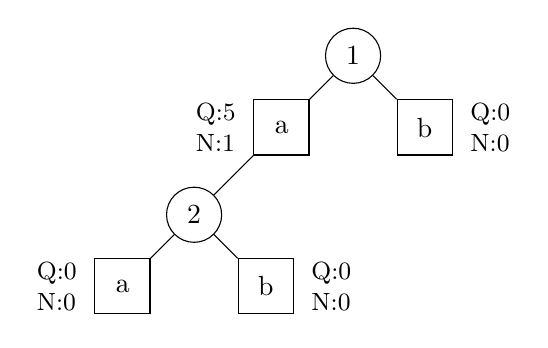
\begin{tikzpicture}
      % Define styles for nodes
      \tikzset{
        circlenode/.style={circle, draw, minimum size=0.7cm, inner sep=0pt},
        squarenode/.style={rectangle, draw, minimum size=0.7cm, inner sep=2pt},
        annotation/.style={font=\small}
      }
      
      % Create the tree structure with the nodes
      \node[circlenode] (node1) {1};
      \node[squarenode, below left=0.3cm and 0.3cm of node1] (nodea1) {a};
      \node[squarenode, below right=0.3cm and 0.3cm of node1] (nodeb1) {b};
      
      \node[circlenode, below left=0.5cm and 0.5cm of nodea1] (node2) {2};
      \node[squarenode, below left=0.3cm and 0.3cm of node2] (nodea2) {a};
      \node[squarenode, below right=0.3cm and 0.3cm of node2] (nodeb2) {b};
      
      % Draw the edges connecting the nodes
      \draw (node1) -- (nodea1);
      \draw (node1) -- (nodeb1);
      \draw (nodea1) -- (node2);
      \draw (node2) -- (nodea2);
      \draw (node2) -- (nodeb2);
      
      % Add annotations next to the nodes
      \node[annotation, left=0.1cm of nodea1, align=left] {Q:5\\N:1};
      \node[annotation, right=0.1cm of nodeb1, align=left] {Q:0\\N:0};
      \node[annotation, left=0.1cm of nodea2, align=left] {Q:0\\N:0};
      \node[annotation, right=0.1cm of nodeb2, align=left] {Q:0\\N:0};
    \end{tikzpicture}
    \end{minipage}
    \begin{minipage}{0.5\textwidth}
        \begin{center}
            G(s, a)\\
            \begin{tabular}{cc|cc}
                \toprule
                $s$ & $a$ & $s'$ & $r$ \\
                \midrule
                1 & a & 2 & 6.0 \\
                1 & b & 3 & 7.0 \\
                2 & a & 4 & 5.0 \\
                2 & b & 4 & 6.0 \\
                \bottomrule
            \end{tabular}
        \end{center}
    \end{minipage}
    \vspace{1cm}
    \begin{enumerate}[label=(\alph*)]
        \item Suppose we run one iteration of MCTS starting from node 1. What is the path of states and actions that the search phase will take including any new state nodes created (e.g. (1, b, 2, b, 5) or (1, a, 4))? Briefly justify why each node is selected.
        \\ \\ \noindent \textbf{Solution: }\\
        MCTS uses the following expression to determine the Upper Confidence Bound (UCB), which is then used to choose actions that maximize the UCB value.
        \begin{equation*}
            \text{UCB}(s,a) = Q(s,a) + c\sqrt{\frac{\log{N(s)}}{N(s,a)}}
        \end{equation*}
        Because $N(s=1,a=\text{b}) = 0$, the UCB value is infinite and the algorithm will choose action $b$ in state 1. From the generative function $G$, $s' = 3$ so the path would be $(1,\text{b},3)$.
        \item Draw any new state and action nodes that would be created in the expansion phase (you can either add to the existing tree or re-draw the tree).
        \\ \\ \noindent \textbf{Solution: }
        \begin{center}
            \begin{minipage}{0.5\textwidth}
    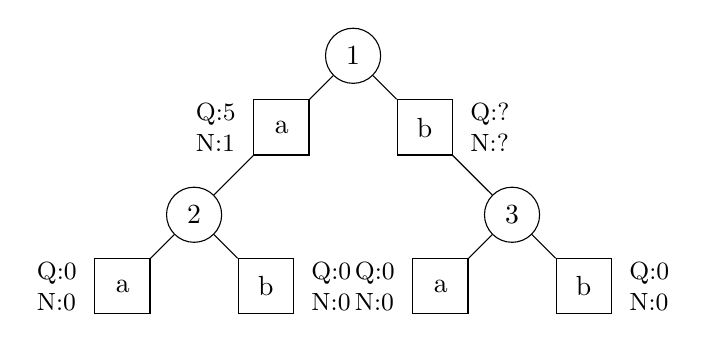
\begin{tikzpicture}
      % Define styles for nodes
      \tikzset{
        circlenode/.style={circle, draw, minimum size=0.7cm, inner sep=0pt},
        squarenode/.style={rectangle, draw, minimum size=0.7cm, inner sep=2pt},
        annotation/.style={font=\small}
      }
      
      % Create the tree structure with the nodes
      \node[circlenode] (node1) {1};
      \node[squarenode, below left=0.3cm and 0.3cm of node1] (nodea1) {a};
      \node[squarenode, below right=0.3cm and 0.3cm of node1] (nodeb1) {b};
      
      \node[circlenode, below left=0.5cm and 0.5cm of nodea1] (node2) {2};
      \node[squarenode, below left=0.3cm and 0.3cm of node2] (nodea2) {a};
      \node[squarenode, below right=0.3cm and 0.3cm of node2] (nodeb2) {b};

      \node[circlenode, below right=0.5cm and 0.5cm of nodeb1] (node3) {3};
      \node[squarenode, below left=0.3cm and 0.3cm of node3] (nodea3) {a};
      \node[squarenode, below right=0.3cm and 0.3cm of node3] (nodeb3) {b};
      
      % Draw the edges connecting the nodes
      \draw (node1) -- (nodea1);
      \draw (node1) -- (nodeb1);
      \draw (nodea1) -- (node2);
      \draw (node2) -- (nodea2);
      \draw (node2) -- (nodeb2);
      \draw (nodeb1) -- (node3);
      \draw (node3) -- (nodea3);
      \draw (node3) -- (nodeb3);
      
      % Add annotations next to the nodes
      \node[annotation, left=0.1cm of nodea1, align=left] {Q:5\\N:1};
      \node[annotation, right=0.1cm of nodeb1, align=left] {Q:?\\N:?};
      \node[annotation, left=0.1cm of nodea2, align=left] {Q:0\\N:0};
      \node[annotation, right=0.1cm of nodeb2, align=left] {Q:0\\N:0};
      \node[annotation, left=0.1cm of nodea3, align=left] {Q:0\\N:0};
      \node[annotation, right=0.1cm of nodeb3, align=left] {Q:0\\N:0};
    \end{tikzpicture}
    \end{minipage}
    \end{center}
    \newpage
        \item Assume the rollout from the new leaf node returns a value estimate of 10. Perform the backup to update the Q and N values at all action nodes nodes on the path (you do not need to copy unchanged values from the existing tree).
        \\ \\ \noindent \textbf{Solution: }\\
        The updated Q value based on the generative function reward and rollout is given below.
    \begin{align*}
        q(s=1,a=\text{b}) &= r(s=1,a = \text{b}) + \gamma\cdot U(3)\\
        &=7 +0.9\cdot10\\
        &= 16\\
        \text{Incrementing N}&\text{ value,}\\
        N(s=1,a=\text{b}) &= 1
    \end{align*}
    Applying to the MCTS Q update,
    \begin{align*}
        Q(s=1,a=\text{b})_{updated} &= Q(s=1,a=\text{b}) + \frac{q(s=1,a=\text{b}) - Q(s=1,a=\text{b})}{N(s=1,a=\text{b})}\\
        &= 0 + \frac{16 - 0}{1} \\
        &= 16\\
    \end{align*}
    \end{enumerate}
\end{question}



\end{document}
